\documentclass[1p]{elsarticle_modified}
%\bibliographystyle{elsarticle-num}

%\usepackage[colorlinks]{hyperref}
%\usepackage{abbrmath_seonhwa} %\Abb, \Ascr, \Acal ,\Abf, \Afrak
\usepackage{amsfonts}
\usepackage{amssymb}
\usepackage{amsmath}
\usepackage{amsthm}
\usepackage{scalefnt}
\usepackage{amsbsy}
\usepackage{kotex}
\usepackage{caption}
\usepackage{subfig}
\usepackage{color}
\usepackage{graphicx}
\usepackage{xcolor} %% white, black, red, green, blue, cyan, magenta, yellow
\usepackage{float}
\usepackage{setspace}
\usepackage{hyperref}

\usepackage{tikz}
\usetikzlibrary{arrows}

\usepackage{multirow}
\usepackage{array} % fixed length table
\usepackage{hhline}

%%%%%%%%%%%%%%%%%%%%%
\makeatletter
\renewcommand*\env@matrix[1][\arraystretch]{%
	\edef\arraystretch{#1}%
	\hskip -\arraycolsep
	\let\@ifnextchar\new@ifnextchar
	\array{*\c@MaxMatrixCols c}}
\makeatother %https://tex.stackexchange.com/questions/14071/how-can-i-increase-the-line-spacing-in-a-matrix
%%%%%%%%%%%%%%%

\usepackage[normalem]{ulem}

\newcommand{\msout}[1]{\ifmmode\text{\sout{\ensuremath{#1}}}\else\sout{#1}\fi}
%SOURCE: \msout is \stkout macro in https://tex.stackexchange.com/questions/20609/strikeout-in-math-mode

\newcommand{\cancel}[1]{
	\ifmmode
	{\color{red}\msout{#1}}
	\else
	{\color{red}\sout{#1}}
	\fi
}

\newcommand{\add}[1]{
	{\color{blue}\uwave{#1}}
}

\newcommand{\replace}[2]{
	\ifmmode
	{\color{red}\msout{#1}}{\color{blue}\uwave{#2}}
	\else
	{\color{red}\sout{#1}}{\color{blue}\uwave{#2}}
	\fi
}

\newcommand{\Sol}{\mathcal{S}} %segment
\newcommand{\D}{D} %diagram
\newcommand{\A}{\mathcal{A}} %arc


%%%%%%%%%%%%%%%%%%%%%%%%%%%%%5 test

\def\sl{\operatorname{\textup{SL}}(2,\Cbb)}
\def\psl{\operatorname{\textup{PSL}}(2,\Cbb)}
\def\quan{\mkern 1mu \triangleright \mkern 1mu}

\theoremstyle{definition}
\newtheorem{thm}{Theorem}[section]
\newtheorem{prop}[thm]{Proposition}
\newtheorem{lem}[thm]{Lemma}
\newtheorem{ques}[thm]{Question}
\newtheorem{cor}[thm]{Corollary}
\newtheorem{defn}[thm]{Definition}
\newtheorem{exam}[thm]{Example}
\newtheorem{rmk}[thm]{Remark}
\newtheorem{alg}[thm]{Algorithm}

\newcommand{\I}{\sqrt{-1}}
\begin{document}

%\begin{frontmatter}
%
%\title{Boundary parabolic representations of knots up to 8 crossings}
%
%%% Group authors per affiliation:
%\author{Yunhi Cho} 
%\address{Department of Mathematics, University of Seoul, Seoul, Korea}
%\ead{yhcho@uos.ac.kr}
%
%
%\author{Seonhwa Kim} %\fnref{s_kim}}
%\address{Center for Geometry and Physics, Institute for Basic Science, Pohang, 37673, Korea}
%\ead{ryeona17@ibs.re.kr}
%
%\author{Hyuk Kim}
%\address{Department of Mathematical Sciences, Seoul National University, Seoul 08826, Korea}
%\ead{hyukkim@snu.ac.kr}
%
%\author{Seokbeom Yoon}
%\address{Department of Mathematical Sciences, Seoul National University, Seoul, 08826,  Korea}
%\ead{sbyoon15@snu.ac.kr}
%
%\begin{abstract}
%We find all boundary parabolic representation of knots up to 8 crossings.
%
%\end{abstract}
%\begin{keyword}
%    \MSC[2010] 57M25 
%\end{keyword}
%
%\end{frontmatter}

%\linenumbers
%\tableofcontents
%
\newcommand\colored[1]{\textcolor{white}{\rule[-0.35ex]{0.8em}{1.4ex}}\kern-0.8em\color{red} #1}%
%\newcommand\colored[1]{\textcolor{white}{ #1}\kern-2.17ex	\textcolor{white}{ #1}\kern-1.81ex	\textcolor{white}{ #1}\kern-2.15ex\color{red}#1	}

{\Large $\underline{12n_{0732}~(K12n_{0732})}$}

\setlength{\tabcolsep}{10pt}
\renewcommand{\arraystretch}{1.6}
\vspace{1cm}\begin{tabular}{m{100pt}>{\centering\arraybackslash}m{274pt}}
\multirow{5}{120pt}{
	\centering
	\includegraphics[width=112pt]{../../../GIT/diagram.site/Diagrams/png/2821_12n_0732.png}\\
\ \ \ A knot diagram\footnotemark}&
\allowdisplaybreaks
\textbf{Linearized knot diagam} \\
\cline{2-2}
 &
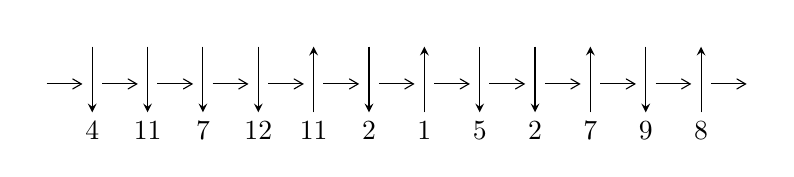
\begin{tikzpicture}[x=20pt, y=17pt]
	% nodes
	\node (C0) at (0, 0) {};
	\node (C1) at (1, 0) {};
	\node (C1U) at (1, +1) {};
	\node (C1D) at (1, -1) {4};

	\node (C2) at (2, 0) {};
	\node (C2U) at (2, +1) {};
	\node (C2D) at (2, -1) {11};

	\node (C3) at (3, 0) {};
	\node (C3U) at (3, +1) {};
	\node (C3D) at (3, -1) {7};

	\node (C4) at (4, 0) {};
	\node (C4U) at (4, +1) {};
	\node (C4D) at (4, -1) {12};

	\node (C5) at (5, 0) {};
	\node (C5U) at (5, +1) {};
	\node (C5D) at (5, -1) {11};

	\node (C6) at (6, 0) {};
	\node (C6U) at (6, +1) {};
	\node (C6D) at (6, -1) {2};

	\node (C7) at (7, 0) {};
	\node (C7U) at (7, +1) {};
	\node (C7D) at (7, -1) {1};

	\node (C8) at (8, 0) {};
	\node (C8U) at (8, +1) {};
	\node (C8D) at (8, -1) {5};

	\node (C9) at (9, 0) {};
	\node (C9U) at (9, +1) {};
	\node (C9D) at (9, -1) {2};

	\node (C10) at (10, 0) {};
	\node (C10U) at (10, +1) {};
	\node (C10D) at (10, -1) {7};

	\node (C11) at (11, 0) {};
	\node (C11U) at (11, +1) {};
	\node (C11D) at (11, -1) {9};

	\node (C12) at (12, 0) {};
	\node (C12U) at (12, +1) {};
	\node (C12D) at (12, -1) {8};
	\node (C13) at (13, 0) {};

	% arrows
	\draw[->,>={angle 60}]
	(C0) edge (C1) (C1) edge (C2) (C2) edge (C3) (C3) edge (C4) (C4) edge (C5) (C5) edge (C6) (C6) edge (C7) (C7) edge (C8) (C8) edge (C9) (C9) edge (C10) (C10) edge (C11) (C11) edge (C12) (C12) edge (C13) ;	\draw[->,>=stealth]
	(C1U) edge (C1D) (C2U) edge (C2D) (C3U) edge (C3D) (C4U) edge (C4D) (C5D) edge (C5U) (C6U) edge (C6D) (C7D) edge (C7U) (C8U) edge (C8D) (C9U) edge (C9D) (C10D) edge (C10U) (C11U) edge (C11D) (C12D) edge (C12U) ;
	\end{tikzpicture} \\
\hhline{~~} \\& 
\textbf{Solving Sequence} \\ \cline{2-2} 
 &
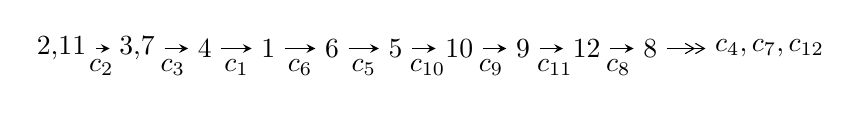
\begin{tikzpicture}[x=23pt, y=7pt]
	% node
	\node (A0) at (-1/8, 0) {2,11};
	\node (A1) at (17/16, 0) {3,7};
	\node (A2) at (17/8, 0) {4};
	\node (A3) at (25/8, 0) {1};
	\node (A4) at (33/8, 0) {6};
	\node (A5) at (41/8, 0) {5};
	\node (A6) at (49/8, 0) {10};
	\node (A7) at (57/8, 0) {9};
	\node (A8) at (65/8, 0) {12};
	\node (A9) at (73/8, 0) {8};
	\node (C1) at (1/2, -1) {$c_{2}$};
	\node (C2) at (13/8, -1) {$c_{3}$};
	\node (C3) at (21/8, -1) {$c_{1}$};
	\node (C4) at (29/8, -1) {$c_{6}$};
	\node (C5) at (37/8, -1) {$c_{5}$};
	\node (C6) at (45/8, -1) {$c_{10}$};
	\node (C7) at (53/8, -1) {$c_{9}$};
	\node (C8) at (61/8, -1) {$c_{11}$};
	\node (C9) at (69/8, -1) {$c_{8}$};
	\node (A10) at (11, 0) {$c_{4},c_{7},c_{12}$};

	% edge
	\draw[->,>=stealth]	
	(A0) edge (A1) (A1) edge (A2) (A2) edge (A3) (A3) edge (A4) (A4) edge (A5) (A5) edge (A6) (A6) edge (A7) (A7) edge (A8) (A8) edge (A9) ;
	\draw[->>,>={angle 60}]	
	(A9) edge (A10);
\end{tikzpicture} \\ 

\end{tabular} \\

\footnotetext{
The image of knot diagram is generated by the software ``\textbf{Draw programme}" developed by Andrew Bartholomew(\url{http://www.layer8.co.uk/maths/draw/index.htm\#Running-draw}), where we modified some parts for our purpose(\url{https://github.com/CATsTAILs/LinksPainter}).
}\phantom \\ \newline 
\centering \textbf{Ideals for irreducible components\footnotemark of $X_{\text{par}}$} 
 
\begin{align*}
I^u_{1}&=\langle 
-3.49919\times10^{429} u^{82}-9.68214\times10^{429} u^{81}+\cdots+4.60228\times10^{434} b+1.01773\times10^{436},\\
\phantom{I^u_{1}}&\phantom{= \langle  }2.05304\times10^{436} u^{82}-7.13618\times10^{435} u^{81}+\cdots+1.09384\times10^{440} a-4.44613\times10^{441},\\
\phantom{I^u_{1}}&\phantom{= \langle  }u^{83}- u^{82}+\cdots+2048046 u-237673\rangle \\
I^u_{2}&=\langle 
3.26221\times10^{19} u^{23}+2.15398\times10^{19} u^{22}+\cdots+1.24108\times10^{19} b+9.39258\times10^{19},\\
\phantom{I^u_{2}}&\phantom{= \langle  }-4.34127\times10^{20} u^{23}-2.45018\times10^{20} u^{22}+\cdots+1.24108\times10^{19} a-9.98705\times10^{20},\;u^{24}+u^{23}+\cdots+4 u+1\rangle \\
I^u_{3}&=\langle 
b- u+1,\;a-1,\;u^2- u+1\rangle \\
\\
\end{align*}
\raggedright * 3 irreducible components of $\dim_{\mathbb{C}}=0$, with total 109 representations.\\
\footnotetext{All coefficients of polynomials are rational numbers. But the coefficients are sometimes approximated in decimal forms when there is not enough margin.}
\newpage
\renewcommand{\arraystretch}{1}
\centering \section*{I. $I^u_{1}= \langle -3.50\times10^{429} u^{82}-9.68\times10^{429} u^{81}+\cdots+4.60\times10^{434} b+1.02\times10^{436},\;2.05\times10^{436} u^{82}-7.14\times10^{435} u^{81}+\cdots+1.09\times10^{440} a-4.45\times10^{441},\;u^{83}- u^{82}+\cdots+2048046 u-237673 \rangle$}
\flushleft \textbf{(i) Arc colorings}\\
\begin{tabular}{m{7pt} m{180pt} m{7pt} m{180pt} }
\flushright $a_{2}=$&$\begin{pmatrix}1\\0\end{pmatrix}$ \\
\flushright $a_{11}=$&$\begin{pmatrix}0\\u\end{pmatrix}$ \\
\flushright $a_{3}=$&$\begin{pmatrix}1\\u^2\end{pmatrix}$ \\
\flushright $a_{7}=$&$\begin{pmatrix}-0.000187692 u^{82}+0.0000652399 u^{81}+\cdots-103.466 u+40.6470\\7.60316\times10^{-6} u^{82}+0.0000210377 u^{81}+\cdots+147.358 u-22.1135\end{pmatrix}$ \\
\flushright $a_{4}=$&$\begin{pmatrix}-0.000163705 u^{82}+0.000162742 u^{81}+\cdots+585.451 u-61.5724\\0.0000442704 u^{82}-0.0000260632 u^{81}+\cdots-70.3579 u+4.73710\end{pmatrix}$ \\
\flushright $a_{1}=$&$\begin{pmatrix}-0.000166790 u^{82}+0.0000820861 u^{81}+\cdots+162.358 u-3.41475\\-0.0000300517 u^{82}+0.0000474903 u^{81}+\cdots+260.800 u-37.0113\end{pmatrix}$ \\
\flushright $a_{6}=$&$\begin{pmatrix}-0.000180088 u^{82}+0.0000862776 u^{81}+\cdots+43.8924 u+18.5335\\7.60316\times10^{-6} u^{82}+0.0000210377 u^{81}+\cdots+147.358 u-22.1135\end{pmatrix}$ \\
\flushright $a_{5}=$&$\begin{pmatrix}-0.000180088 u^{82}+0.0000862776 u^{81}+\cdots+43.8924 u+18.5335\\0.0000152790 u^{82}+0.0000407085 u^{81}+\cdots+296.685 u-44.4098\end{pmatrix}$ \\
\flushright $a_{10}=$&$\begin{pmatrix}-0.000281266 u^{82}+0.000174152 u^{81}+\cdots+380.064 u-13.2873\\0.0000201427 u^{82}-0.0000310990 u^{81}+\cdots-119.176 u+13.4499\end{pmatrix}$ \\
\flushright $a_{9}=$&$\begin{pmatrix}-0.000261124 u^{82}+0.000143053 u^{81}+\cdots+260.888 u+0.162624\\0.0000201427 u^{82}-0.0000310990 u^{81}+\cdots-119.176 u+13.4499\end{pmatrix}$ \\
\flushright $a_{12}=$&$\begin{pmatrix}0.000334705 u^{82}-0.000159389 u^{81}+\cdots-166.178 u-24.0662\\-0.0000280200 u^{82}-0.0000248455 u^{81}+\cdots-290.374 u+47.0998\end{pmatrix}$ \\
\flushright $a_{8}=$&$\begin{pmatrix}-0.000362649 u^{82}+0.000164944 u^{81}+\cdots+185.086 u+25.2579\\-0.0000348471 u^{82}+0.0000542533 u^{81}+\cdots+337.625 u-45.7974\end{pmatrix}$\\&\end{tabular}
\flushleft \textbf{(ii) Obstruction class $= -1$}\\~\\
\flushleft \textbf{(iii) Cusp Shapes $= -0.000301960 u^{82}+0.000391858 u^{81}+\cdots+1897.38 u-240.107$}\\~\\
\newpage\renewcommand{\arraystretch}{1}
\flushleft \textbf{(iv) u-Polynomials at the component}\newline \\
\begin{tabular}{m{50pt}|m{274pt}}
Crossings & \hspace{64pt}u-Polynomials at each crossing \\
\hline $$\begin{aligned}c_{1}\end{aligned}$$&$\begin{aligned}
&u^{83}-11 u^{82}+\cdots-3341 u+203
\end{aligned}$\\
\hline $$\begin{aligned}c_{2}\end{aligned}$$&$\begin{aligned}
&u^{83}+u^{82}+\cdots+2048046 u+237673
\end{aligned}$\\
\hline $$\begin{aligned}c_{3}\end{aligned}$$&$\begin{aligned}
&u^{83}+u^{82}+\cdots-15388 u+2108
\end{aligned}$\\
\hline $$\begin{aligned}c_{4}\end{aligned}$$&$\begin{aligned}
&u^{83}+3 u^{82}+\cdots-16 u+1
\end{aligned}$\\
\hline $$\begin{aligned}c_{5}\end{aligned}$$&$\begin{aligned}
&u^{83}-15 u^{81}+\cdots-663559 u+83839
\end{aligned}$\\
\hline $$\begin{aligned}c_{6}\end{aligned}$$&$\begin{aligned}
&u^{83}+5 u^{82}+\cdots+97593 u+5351
\end{aligned}$\\
\hline $$\begin{aligned}c_{7},c_{12}\end{aligned}$$&$\begin{aligned}
&u^{83}-3 u^{82}+\cdots+1495 u+103
\end{aligned}$\\
\hline $$\begin{aligned}c_{8}\end{aligned}$$&$\begin{aligned}
&u^{83}+6 u^{82}+\cdots+322 u+29
\end{aligned}$\\
\hline $$\begin{aligned}c_{9}\end{aligned}$$&$\begin{aligned}
&u^{83}-3 u^{82}+\cdots+23642902 u+6207563
\end{aligned}$\\
\hline $$\begin{aligned}c_{10}\end{aligned}$$&$\begin{aligned}
&u^{83}-2 u^{82}+\cdots+130300 u+11257
\end{aligned}$\\
\hline $$\begin{aligned}c_{11}\end{aligned}$$&$\begin{aligned}
&u^{83}-12 u^{82}+\cdots-12 u+1
\end{aligned}$\\
\hline
\end{tabular}\\~\\
\newpage\renewcommand{\arraystretch}{1}
\flushleft \textbf{(v) Riley Polynomials at the component}\newline \\
\begin{tabular}{m{50pt}|m{274pt}}
Crossings & \hspace{64pt}Riley Polynomials at each crossing \\
\hline $$\begin{aligned}c_{1}\end{aligned}$$&$\begin{aligned}
&y^{83}+5 y^{82}+\cdots-397351 y-41209
\end{aligned}$\\
\hline $$\begin{aligned}c_{2}\end{aligned}$$&$\begin{aligned}
&y^{83}+93 y^{82}+\cdots-1365124926432 y-56488454929
\end{aligned}$\\
\hline $$\begin{aligned}c_{3}\end{aligned}$$&$\begin{aligned}
&y^{83}+15 y^{82}+\cdots-56398528 y-4443664
\end{aligned}$\\
\hline $$\begin{aligned}c_{4}\end{aligned}$$&$\begin{aligned}
&y^{83}-11 y^{82}+\cdots+50 y-1
\end{aligned}$\\
\hline $$\begin{aligned}c_{5}\end{aligned}$$&$\begin{aligned}
&y^{83}-30 y^{82}+\cdots+63722693959 y-7028977921
\end{aligned}$\\
\hline $$\begin{aligned}c_{6}\end{aligned}$$&$\begin{aligned}
&y^{83}+97 y^{82}+\cdots-743094449 y-28633201
\end{aligned}$\\
\hline $$\begin{aligned}c_{7},c_{12}\end{aligned}$$&$\begin{aligned}
&y^{83}+59 y^{82}+\cdots-208547 y-10609
\end{aligned}$\\
\hline $$\begin{aligned}c_{8}\end{aligned}$$&$\begin{aligned}
&y^{83}-12 y^{82}+\cdots+29850 y-841
\end{aligned}$\\
\hline $$\begin{aligned}c_{9}\end{aligned}$$&$\begin{aligned}
&y^{83}+53 y^{82}+\cdots-759411803692702 y-38533838398969
\end{aligned}$\\
\hline $$\begin{aligned}c_{10}\end{aligned}$$&$\begin{aligned}
&y^{83}-98 y^{82}+\cdots+5637157808 y-126720049
\end{aligned}$\\
\hline $$\begin{aligned}c_{11}\end{aligned}$$&$\begin{aligned}
&y^{83}+22 y^{82}+\cdots+68 y-1
\end{aligned}$\\
\hline
\end{tabular}\\~\\
\newpage\flushleft \textbf{(vi) Complex Volumes and Cusp Shapes}
$$\begin{array}{c|c|c}  
\text{Solutions to }I^u_{1}& \I (\text{vol} + \sqrt{-1}CS) & \text{Cusp shape}\\
 \hline 
\begin{aligned}
u &= \phantom{-}0.414352 + 0.904844 I \\
a &= \phantom{-}0.818742 - 0.835049 I \\
b &= -0.234982 + 1.126650 I\end{aligned}
 & -0.50253 - 2.71042 I & \phantom{-0.000000 } 0 \\ \hline\begin{aligned}
u &= \phantom{-}0.414352 - 0.904844 I \\
a &= \phantom{-}0.818742 + 0.835049 I \\
b &= -0.234982 - 1.126650 I\end{aligned}
 & -0.50253 + 2.71042 I & \phantom{-0.000000 } 0 \\ \hline\begin{aligned}
u &= -1.028260 + 0.017055 I \\
a &= \phantom{-}0.537212 + 0.257597 I \\
b &= \phantom{-}1.340570 - 0.138864 I\end{aligned}
 & -4.09989 + 1.06646 I & \phantom{-0.000000 } 0 \\ \hline\begin{aligned}
u &= -1.028260 - 0.017055 I \\
a &= \phantom{-}0.537212 - 0.257597 I \\
b &= \phantom{-}1.340570 + 0.138864 I\end{aligned}
 & -4.09989 - 1.06646 I & \phantom{-0.000000 } 0 \\ \hline\begin{aligned}
u &= \phantom{-}0.417263 + 0.866402 I \\
a &= \phantom{-}0.318885 - 0.410092 I \\
b &= -1.098590 + 0.129272 I\end{aligned}
 & -3.34845 - 4.34438 I & \phantom{-0.000000 -}0. + 7.77500 I \\ \hline\begin{aligned}
u &= \phantom{-}0.417263 - 0.866402 I \\
a &= \phantom{-}0.318885 + 0.410092 I \\
b &= -1.098590 - 0.129272 I\end{aligned}
 & -3.34845 + 4.34438 I & \phantom{-0.000000 } 0. - 7.77500 I \\ \hline\begin{aligned}
u &= -0.572659 + 0.744013 I \\
a &= \phantom{-}0.505280 - 0.031757 I \\
b &= \phantom{-}1.191840 + 0.333632 I\end{aligned}
 & -4.39495 - 1.29965 I & -4.00000 + 3.00721 I \\ \hline\begin{aligned}
u &= -0.572659 - 0.744013 I \\
a &= \phantom{-}0.505280 + 0.031757 I \\
b &= \phantom{-}1.191840 - 0.333632 I\end{aligned}
 & -4.39495 + 1.29965 I & -4.00000 - 3.00721 I \\ \hline\begin{aligned}
u &= -1.040930 + 0.307428 I \\
a &= -0.273096 - 0.755471 I \\
b &= \phantom{-}0.451724 + 0.662973 I\end{aligned}
 & -3.60574 - 2.70826 I & \phantom{-0.000000 } 0 \\ \hline\begin{aligned}
u &= -1.040930 - 0.307428 I \\
a &= -0.273096 + 0.755471 I \\
b &= \phantom{-}0.451724 - 0.662973 I\end{aligned}
 & -3.60574 + 2.70826 I & \phantom{-0.000000 } 0\\
 \hline 
 \end{array}$$\newpage$$\begin{array}{c|c|c}  
\text{Solutions to }I^u_{1}& \I (\text{vol} + \sqrt{-1}CS) & \text{Cusp shape}\\
 \hline 
\begin{aligned}
u &= \phantom{-}0.637570 + 0.910156 I \\
a &= \phantom{-}1.063740 + 0.356958 I \\
b &= \phantom{-}0.347803 - 0.186767 I\end{aligned}
 & -4.05843 + 0.77081 I & \phantom{-0.000000 } 0 \\ \hline\begin{aligned}
u &= \phantom{-}0.637570 - 0.910156 I \\
a &= \phantom{-}1.063740 - 0.356958 I \\
b &= \phantom{-}0.347803 + 0.186767 I\end{aligned}
 & -4.05843 - 0.77081 I & \phantom{-0.000000 } 0 \\ \hline\begin{aligned}
u &= \phantom{-}0.177985 + 1.106920 I \\
a &= \phantom{-}0.489709 - 1.232370 I \\
b &= -0.21437 + 1.49408 I\end{aligned}
 & -0.48146 - 2.63965 I & \phantom{-0.000000 } 0 \\ \hline\begin{aligned}
u &= \phantom{-}0.177985 - 1.106920 I \\
a &= \phantom{-}0.489709 + 1.232370 I \\
b &= -0.21437 - 1.49408 I\end{aligned}
 & -0.48146 + 2.63965 I & \phantom{-0.000000 } 0 \\ \hline\begin{aligned}
u &= \phantom{-}0.671577 + 0.559435 I \\
a &= -0.79653 - 1.25063 I \\
b &= \phantom{-}0.100737 + 0.378624 I\end{aligned}
 & -4.38490 + 1.02535 I & -8.49512 + 1.62379 I \\ \hline\begin{aligned}
u &= \phantom{-}0.671577 - 0.559435 I \\
a &= -0.79653 + 1.25063 I \\
b &= \phantom{-}0.100737 - 0.378624 I\end{aligned}
 & -4.38490 - 1.02535 I & -8.49512 - 1.62379 I \\ \hline\begin{aligned}
u &= -0.345440 + 0.798324 I \\
a &= -1.81170 - 0.41097 I \\
b &= \phantom{-}1.42764 + 1.03205 I\end{aligned}
 & -0.93031 + 4.30963 I & -10.3870 - 14.3250 I \\ \hline\begin{aligned}
u &= -0.345440 - 0.798324 I \\
a &= -1.81170 + 0.41097 I \\
b &= \phantom{-}1.42764 - 1.03205 I\end{aligned}
 & -0.93031 - 4.30963 I & -10.3870 + 14.3250 I \\ \hline\begin{aligned}
u &= -0.301371 + 0.752449 I \\
a &= -1.98642 + 0.02905 I \\
b &= \phantom{-}0.321899 - 0.106934 I\end{aligned}
 & -3.76643 - 9.37621 I & -3.18784 + 5.46497 I \\ \hline\begin{aligned}
u &= -0.301371 - 0.752449 I \\
a &= -1.98642 - 0.02905 I \\
b &= \phantom{-}0.321899 + 0.106934 I\end{aligned}
 & -3.76643 + 9.37621 I & -3.18784 - 5.46497 I\\
 \hline 
 \end{array}$$\newpage$$\begin{array}{c|c|c}  
\text{Solutions to }I^u_{1}& \I (\text{vol} + \sqrt{-1}CS) & \text{Cusp shape}\\
 \hline 
\begin{aligned}
u &= \phantom{-}0.773390 + 0.175831 I \\
a &= \phantom{-}0.369949 - 0.128530 I \\
b &= \phantom{-}0.794235 - 0.233534 I\end{aligned}
 & -1.178940 - 0.026902 I & -2.24486 - 0.66294 I \\ \hline\begin{aligned}
u &= \phantom{-}0.773390 - 0.175831 I \\
a &= \phantom{-}0.369949 + 0.128530 I \\
b &= \phantom{-}0.794235 + 0.233534 I\end{aligned}
 & -1.178940 + 0.026902 I & -2.24486 + 0.66294 I \\ \hline\begin{aligned}
u &= \phantom{-}0.379090 + 0.679111 I \\
a &= \phantom{-}0.310084 + 0.343934 I \\
b &= -1.53351 + 0.59005 I\end{aligned}
 & -4.03656 + 9.14747 I & -3.08929 - 4.48071 I \\ \hline\begin{aligned}
u &= \phantom{-}0.379090 - 0.679111 I \\
a &= \phantom{-}0.310084 - 0.343934 I \\
b &= -1.53351 - 0.59005 I\end{aligned}
 & -4.03656 - 9.14747 I & -3.08929 + 4.48071 I \\ \hline\begin{aligned}
u &= -0.585406 + 1.076470 I \\
a &= \phantom{-}0.769362 - 0.107344 I \\
b &= \phantom{-}0.067450 - 0.608539 I\end{aligned}
 & -1.13069 + 3.60924 I & \phantom{-0.000000 } 0 \\ \hline\begin{aligned}
u &= -0.585406 - 1.076470 I \\
a &= \phantom{-}0.769362 + 0.107344 I \\
b &= \phantom{-}0.067450 + 0.608539 I\end{aligned}
 & -1.13069 - 3.60924 I & \phantom{-0.000000 } 0 \\ \hline\begin{aligned}
u &= -0.608231 + 0.426041 I \\
a &= \phantom{-}0.659662 + 0.542829 I \\
b &= -0.184618 + 0.399153 I\end{aligned}
 & \phantom{-}2.56481 + 0.56873 I & \phantom{-}1.41112 - 2.57174 I \\ \hline\begin{aligned}
u &= -0.608231 - 0.426041 I \\
a &= \phantom{-}0.659662 - 0.542829 I \\
b &= -0.184618 - 0.399153 I\end{aligned}
 & \phantom{-}2.56481 - 0.56873 I & \phantom{-}1.41112 + 2.57174 I \\ \hline\begin{aligned}
u &= \phantom{-}1.064550 + 0.709606 I \\
a &= \phantom{-}0.526848 - 0.134656 I \\
b &= \phantom{-}0.134105 + 0.347107 I\end{aligned}
 & -2.03220 - 2.79313 I & \phantom{-0.000000 } 0 \\ \hline\begin{aligned}
u &= \phantom{-}1.064550 - 0.709606 I \\
a &= \phantom{-}0.526848 + 0.134656 I \\
b &= \phantom{-}0.134105 - 0.347107 I\end{aligned}
 & -2.03220 + 2.79313 I & \phantom{-0.000000 } 0\\
 \hline 
 \end{array}$$\newpage$$\begin{array}{c|c|c}  
\text{Solutions to }I^u_{1}& \I (\text{vol} + \sqrt{-1}CS) & \text{Cusp shape}\\
 \hline 
\begin{aligned}
u &= -1.166100 + 0.526433 I \\
a &= -0.305083 + 0.019879 I \\
b &= -0.220833 - 0.594073 I\end{aligned}
 & \phantom{-}1.82630 + 4.81831 I & \phantom{-0.000000 } 0 \\ \hline\begin{aligned}
u &= -1.166100 - 0.526433 I \\
a &= -0.305083 - 0.019879 I \\
b &= -0.220833 + 0.594073 I\end{aligned}
 & \phantom{-}1.82630 - 4.81831 I & \phantom{-0.000000 } 0 \\ \hline\begin{aligned}
u &= -0.205221 + 0.687069 I \\
a &= \phantom{-}0.768610 - 0.379877 I \\
b &= -1.303500 - 0.456175 I\end{aligned}
 & \phantom{-}1.29077 - 3.56733 I & \phantom{-}1.02756 + 5.38922 I \\ \hline\begin{aligned}
u &= -0.205221 - 0.687069 I \\
a &= \phantom{-}0.768610 + 0.379877 I \\
b &= -1.303500 + 0.456175 I\end{aligned}
 & \phantom{-}1.29077 + 3.56733 I & \phantom{-}1.02756 - 5.38922 I \\ \hline\begin{aligned}
u &= -1.239500 + 0.371890 I \\
a &= \phantom{-}0.651770 - 0.371480 I \\
b &= \phantom{-}0.435731 + 0.296635 I\end{aligned}
 & -3.67543 - 1.63059 I & \phantom{-0.000000 } 0 \\ \hline\begin{aligned}
u &= -1.239500 - 0.371890 I \\
a &= \phantom{-}0.651770 + 0.371480 I \\
b &= \phantom{-}0.435731 - 0.296635 I\end{aligned}
 & -3.67543 + 1.63059 I & \phantom{-0.000000 } 0 \\ \hline\begin{aligned}
u &= \phantom{-}0.692399 + 0.077190 I \\
a &= \phantom{-}1.163320 - 0.065011 I \\
b &= \phantom{-}0.158615 - 0.881612 I\end{aligned}
 & -0.69388 + 3.26055 I & -4.25295 - 4.21550 I \\ \hline\begin{aligned}
u &= \phantom{-}0.692399 - 0.077190 I \\
a &= \phantom{-}1.163320 + 0.065011 I \\
b &= \phantom{-}0.158615 + 0.881612 I\end{aligned}
 & -0.69388 - 3.26055 I & -4.25295 + 4.21550 I \\ \hline\begin{aligned}
u &= \phantom{-}0.422423 + 1.314500 I \\
a &= -0.553764 + 1.137490 I \\
b &= -0.34607 - 1.85608 I\end{aligned}
 & \phantom{-}4.09935 - 1.72757 I & \phantom{-0.000000 } 0 \\ \hline\begin{aligned}
u &= \phantom{-}0.422423 - 1.314500 I \\
a &= -0.553764 - 1.137490 I \\
b &= -0.34607 + 1.85608 I\end{aligned}
 & \phantom{-}4.09935 + 1.72757 I & \phantom{-0.000000 } 0\\
 \hline 
 \end{array}$$\newpage$$\begin{array}{c|c|c}  
\text{Solutions to }I^u_{1}& \I (\text{vol} + \sqrt{-1}CS) & \text{Cusp shape}\\
 \hline 
\begin{aligned}
u &= \phantom{-}0.591218\phantom{ +0.000000I} \\
a &= \phantom{-}0.492574\phantom{ +0.000000I} \\
b &= \phantom{-}0.792557\phantom{ +0.000000I}\end{aligned}
 & -1.19065\phantom{ +0.000000I} & -5.17470\phantom{ +0.000000I} \\ \hline\begin{aligned}
u &= \phantom{-}0.46810 + 1.33998 I \\
a &= \phantom{-}0.109017 - 1.294080 I \\
b &= -0.29965 + 1.64714 I\end{aligned}
 & \phantom{-}5.93412 - 1.92291 I & \phantom{-0.000000 } 0 \\ \hline\begin{aligned}
u &= \phantom{-}0.46810 - 1.33998 I \\
a &= \phantom{-}0.109017 + 1.294080 I \\
b &= -0.29965 - 1.64714 I\end{aligned}
 & \phantom{-}5.93412 + 1.92291 I & \phantom{-0.000000 } 0 \\ \hline\begin{aligned}
u &= -0.039654 + 0.574075 I \\
a &= \phantom{-}1.55657 + 0.40480 I \\
b &= -0.354654 + 0.415931 I\end{aligned}
 & \phantom{-}0.25628 - 1.95793 I & \phantom{-}0.76700 + 3.94410 I \\ \hline\begin{aligned}
u &= -0.039654 - 0.574075 I \\
a &= \phantom{-}1.55657 - 0.40480 I \\
b &= -0.354654 - 0.415931 I\end{aligned}
 & \phantom{-}0.25628 + 1.95793 I & \phantom{-}0.76700 - 3.94410 I \\ \hline\begin{aligned}
u &= \phantom{-}0.09161 + 1.49038 I \\
a &= \phantom{-}0.157174 + 1.324810 I \\
b &= -0.70464 - 1.82638 I\end{aligned}
 & \phantom{-}5.65852 - 3.30039 I & \phantom{-0.000000 } 0 \\ \hline\begin{aligned}
u &= \phantom{-}0.09161 - 1.49038 I \\
a &= \phantom{-}0.157174 - 1.324810 I \\
b &= -0.70464 + 1.82638 I\end{aligned}
 & \phantom{-}5.65852 + 3.30039 I & \phantom{-0.000000 } 0 \\ \hline\begin{aligned}
u &= \phantom{-}0.202641 + 0.448566 I \\
a &= -2.95926 - 0.10425 I \\
b &= \phantom{-}0.689201 + 0.115151 I\end{aligned}
 & \phantom{-}0.45787 + 3.68682 I & \phantom{-}1.09725 - 1.38698 I \\ \hline\begin{aligned}
u &= \phantom{-}0.202641 - 0.448566 I \\
a &= -2.95926 + 0.10425 I \\
b &= \phantom{-}0.689201 - 0.115151 I\end{aligned}
 & \phantom{-}0.45787 - 3.68682 I & \phantom{-}1.09725 + 1.38698 I \\ \hline\begin{aligned}
u &= \phantom{-}0.330652 + 0.359921 I \\
a &= \phantom{-}1.81179 - 0.11132 I \\
b &= \phantom{-}1.141310 + 0.719359 I\end{aligned}
 & -2.58496 - 1.33025 I & -4.54267 + 0.24463 I\\
 \hline 
 \end{array}$$\newpage$$\begin{array}{c|c|c}  
\text{Solutions to }I^u_{1}& \I (\text{vol} + \sqrt{-1}CS) & \text{Cusp shape}\\
 \hline 
\begin{aligned}
u &= \phantom{-}0.330652 - 0.359921 I \\
a &= \phantom{-}1.81179 + 0.11132 I \\
b &= \phantom{-}1.141310 - 0.719359 I\end{aligned}
 & -2.58496 + 1.33025 I & -4.54267 - 0.24463 I \\ \hline\begin{aligned}
u &= \phantom{-}1.47401 + 0.34353 I \\
a &= -0.530455 - 0.057065 I \\
b &= -0.327942 + 0.676870 I\end{aligned}
 & -2.11190 - 9.30846 I & \phantom{-0.000000 } 0 \\ \hline\begin{aligned}
u &= \phantom{-}1.47401 - 0.34353 I \\
a &= -0.530455 + 0.057065 I \\
b &= -0.327942 - 0.676870 I\end{aligned}
 & -2.11190 + 9.30846 I & \phantom{-0.000000 } 0 \\ \hline\begin{aligned}
u &= \phantom{-}0.236925 + 0.417535 I \\
a &= \phantom{-}1.25133 + 1.31707 I \\
b &= \phantom{-}0.011013 + 0.527287 I\end{aligned}
 & -0.39541 - 2.01429 I & -2.84666 + 4.46361 I \\ \hline\begin{aligned}
u &= \phantom{-}0.236925 - 0.417535 I \\
a &= \phantom{-}1.25133 - 1.31707 I \\
b &= \phantom{-}0.011013 - 0.527287 I\end{aligned}
 & -0.39541 + 2.01429 I & -2.84666 - 4.46361 I \\ \hline\begin{aligned}
u &= -0.21429 + 1.55945 I \\
a &= -0.084526 + 1.258460 I \\
b &= \phantom{-}0.28263 - 2.02678 I\end{aligned}
 & \phantom{-}8.82612 + 3.64300 I & \phantom{-0.000000 } 0 \\ \hline\begin{aligned}
u &= -0.21429 - 1.55945 I \\
a &= -0.084526 - 1.258460 I \\
b &= \phantom{-}0.28263 + 2.02678 I\end{aligned}
 & \phantom{-}8.82612 - 3.64300 I & \phantom{-0.000000 } 0 \\ \hline\begin{aligned}
u &= -0.32416 + 1.63100 I \\
a &= \phantom{-}0.089654 + 1.094170 I \\
b &= -0.26089 - 1.69470 I\end{aligned}
 & \phantom{-}6.91762 + 0.07901 I & \phantom{-0.000000 } 0 \\ \hline\begin{aligned}
u &= -0.32416 - 1.63100 I \\
a &= \phantom{-}0.089654 - 1.094170 I \\
b &= -0.26089 + 1.69470 I\end{aligned}
 & \phantom{-}6.91762 - 0.07901 I & \phantom{-0.000000 } 0 \\ \hline\begin{aligned}
u &= \phantom{-}0.06848 + 1.67430 I \\
a &= \phantom{-}0.135743 + 1.110070 I \\
b &= -0.22960 - 1.48707 I\end{aligned}
 & \phantom{-}5.24143 - 2.04516 I & \phantom{-0.000000 } 0\\
 \hline 
 \end{array}$$\newpage$$\begin{array}{c|c|c}  
\text{Solutions to }I^u_{1}& \I (\text{vol} + \sqrt{-1}CS) & \text{Cusp shape}\\
 \hline 
\begin{aligned}
u &= \phantom{-}0.06848 - 1.67430 I \\
a &= \phantom{-}0.135743 - 1.110070 I \\
b &= -0.22960 + 1.48707 I\end{aligned}
 & \phantom{-}5.24143 + 2.04516 I & \phantom{-0.000000 } 0 \\ \hline\begin{aligned}
u &= -0.43500 + 1.67959 I \\
a &= \phantom{-}0.032353 - 1.130650 I \\
b &= -0.15356 + 1.52921 I\end{aligned}
 & \phantom{-}1.75253 + 8.69397 I & \phantom{-0.000000 } 0 \\ \hline\begin{aligned}
u &= -0.43500 - 1.67959 I \\
a &= \phantom{-}0.032353 + 1.130650 I \\
b &= -0.15356 - 1.52921 I\end{aligned}
 & \phantom{-}1.75253 - 8.69397 I & \phantom{-0.000000 } 0 \\ \hline\begin{aligned}
u &= -0.38585 + 1.74072 I \\
a &= \phantom{-}0.098702 + 0.779884 I \\
b &= \phantom{-}0.56146 - 1.98339 I\end{aligned}
 & \phantom{-}2.44247 + 7.16275 I & \phantom{-0.000000 } 0 \\ \hline\begin{aligned}
u &= -0.38585 - 1.74072 I \\
a &= \phantom{-}0.098702 - 0.779884 I \\
b &= \phantom{-}0.56146 + 1.98339 I\end{aligned}
 & \phantom{-}2.44247 - 7.16275 I & \phantom{-0.000000 } 0 \\ \hline\begin{aligned}
u &= -0.19041 + 1.78225 I \\
a &= -0.262423 - 0.898122 I \\
b &= -0.34219 + 1.82899 I\end{aligned}
 & \phantom{-}9.74534 - 1.33402 I & \phantom{-0.000000 } 0 \\ \hline\begin{aligned}
u &= -0.19041 - 1.78225 I \\
a &= -0.262423 + 0.898122 I \\
b &= -0.34219 - 1.82899 I\end{aligned}
 & \phantom{-}9.74534 + 1.33402 I & \phantom{-0.000000 } 0 \\ \hline\begin{aligned}
u &= -0.41279 + 1.75000 I \\
a &= -0.056811 - 1.110350 I \\
b &= -0.45263 + 1.93300 I\end{aligned}
 & \phantom{-}9.4871 + 10.9918 I & \phantom{-0.000000 } 0 \\ \hline\begin{aligned}
u &= -0.41279 - 1.75000 I \\
a &= -0.056811 + 1.110350 I \\
b &= -0.45263 - 1.93300 I\end{aligned}
 & \phantom{-}9.4871 - 10.9918 I & \phantom{-0.000000 } 0 \\ \hline\begin{aligned}
u &= \phantom{-}0.21850 + 1.80286 I \\
a &= \phantom{-}0.150227 + 0.988006 I \\
b &= \phantom{-}0.37037 - 1.50853 I\end{aligned}
 & \phantom{-}8.03484 + 1.01421 I & \phantom{-0.000000 } 0\\
 \hline 
 \end{array}$$\newpage$$\begin{array}{c|c|c}  
\text{Solutions to }I^u_{1}& \I (\text{vol} + \sqrt{-1}CS) & \text{Cusp shape}\\
 \hline 
\begin{aligned}
u &= \phantom{-}0.21850 - 1.80286 I \\
a &= \phantom{-}0.150227 - 0.988006 I \\
b &= \phantom{-}0.37037 + 1.50853 I\end{aligned}
 & \phantom{-}8.03484 - 1.01421 I & \phantom{-0.000000 } 0 \\ \hline\begin{aligned}
u &= \phantom{-}0.26361 + 1.80476 I \\
a &= -0.127641 - 0.996713 I \\
b &= \phantom{-}0.29776 + 1.98890 I\end{aligned}
 & \phantom{-}7.10818 - 8.02637 I & \phantom{-0.000000 } 0 \\ \hline\begin{aligned}
u &= \phantom{-}0.26361 - 1.80476 I \\
a &= -0.127641 + 0.996713 I \\
b &= \phantom{-}0.29776 - 1.98890 I\end{aligned}
 & \phantom{-}7.10818 + 8.02637 I & \phantom{-0.000000 } 0 \\ \hline\begin{aligned}
u &= \phantom{-}0.58577 + 1.80045 I \\
a &= -0.096228 + 1.043080 I \\
b &= -0.42567 - 1.97742 I\end{aligned}
 & \phantom{-}4.7687 - 17.1701 I & \phantom{-0.000000 } 0 \\ \hline\begin{aligned}
u &= \phantom{-}0.58577 - 1.80045 I \\
a &= -0.096228 - 1.043080 I \\
b &= -0.42567 + 1.97742 I\end{aligned}
 & \phantom{-}4.7687 + 17.1701 I & \phantom{-0.000000 } 0 \\ \hline\begin{aligned}
u &= \phantom{-}0.39418 + 1.91028 I \\
a &= \phantom{-}0.097542 - 0.907782 I \\
b &= \phantom{-}0.34950 + 1.88034 I\end{aligned}
 & \phantom{-}6.81458 - 5.87576 I & \phantom{-0.000000 } 0 \\ \hline\begin{aligned}
u &= \phantom{-}0.39418 - 1.91028 I \\
a &= \phantom{-}0.097542 + 0.907782 I \\
b &= \phantom{-}0.34950 - 1.88034 I\end{aligned}
 & \phantom{-}6.81458 + 5.87576 I & \phantom{-0.000000 } 0 \\ \hline\begin{aligned}
u &= \phantom{-}0.10550 + 2.05313 I \\
a &= \phantom{-}0.113249 - 0.915035 I \\
b &= \phantom{-}0.32092 + 1.73513 I\end{aligned}
 & \phantom{-}7.40347 - 6.14595 I & \phantom{-0.000000 } 0 \\ \hline\begin{aligned}
u &= \phantom{-}0.10550 - 2.05313 I \\
a &= \phantom{-}0.113249 + 0.915035 I \\
b &= \phantom{-}0.32092 - 1.73513 I\end{aligned}
 & \phantom{-}7.40347 + 6.14595 I & \phantom{-0.000000 } 0 \\ \hline\begin{aligned}
u &= -0.02637 + 2.06647 I \\
a &= -0.139226 + 0.783931 I \\
b &= -0.28831 - 1.90761 I\end{aligned}
 & \phantom{-}6.56568 + 5.36669 I & \phantom{-0.000000 } 0\\
 \hline 
 \end{array}$$\newpage$$\begin{array}{c|c|c}  
\text{Solutions to }I^u_{1}& \I (\text{vol} + \sqrt{-1}CS) & \text{Cusp shape}\\
 \hline 
\begin{aligned}
u &= -0.02637 - 2.06647 I \\
a &= -0.139226 - 0.783931 I \\
b &= -0.28831 + 1.90761 I\end{aligned}
 & \phantom{-}6.56568 - 5.36669 I & \phantom{-0.000000 } 0 \\ \hline\begin{aligned}
u &= -0.76454 + 1.92604 I \\
a &= \phantom{-}0.178371 + 0.912927 I \\
b &= \phantom{-}0.28342 - 1.88805 I\end{aligned}
 & \phantom{-}4.14225 + 7.38613 I & \phantom{-0.000000 } 0 \\ \hline\begin{aligned}
u &= -0.76454 - 1.92604 I \\
a &= \phantom{-}0.178371 - 0.912927 I \\
b &= \phantom{-}0.28342 + 1.88805 I\end{aligned}
 & \phantom{-}4.14225 - 7.38613 I & \phantom{-0.000000 } 0\\
 \hline 
 \end{array}$$\newpage\newpage\renewcommand{\arraystretch}{1}
\centering \section*{II. $I^u_{2}= \langle 3.26\times10^{19} u^{23}+2.15\times10^{19} u^{22}+\cdots+1.24\times10^{19} b+9.39\times10^{19},\;-4.34\times10^{20} u^{23}-2.45\times10^{20} u^{22}+\cdots+1.24\times10^{19} a-9.99\times10^{20},\;u^{24}+u^{23}+\cdots+4 u+1 \rangle$}
\flushleft \textbf{(i) Arc colorings}\\
\begin{tabular}{m{7pt} m{180pt} m{7pt} m{180pt} }
\flushright $a_{2}=$&$\begin{pmatrix}1\\0\end{pmatrix}$ \\
\flushright $a_{11}=$&$\begin{pmatrix}0\\u\end{pmatrix}$ \\
\flushright $a_{3}=$&$\begin{pmatrix}1\\u^2\end{pmatrix}$ \\
\flushright $a_{7}=$&$\begin{pmatrix}34.9798 u^{23}+19.7424 u^{22}+\cdots+137.849 u+80.4708\\-2.62853 u^{23}-1.73557 u^{22}+\cdots-10.2826 u-7.56808\end{pmatrix}$ \\
\flushright $a_{4}=$&$\begin{pmatrix}-28.5351 u^{23}-15.9884 u^{22}+\cdots-112.157 u-63.1806\\13.4031 u^{23}+7.72081 u^{22}+\cdots+51.6847 u+31.9247\end{pmatrix}$ \\
\flushright $a_{1}=$&$\begin{pmatrix}-7.56905 u^{23}-4.96424 u^{22}+\cdots-27.4653 u-21.4742\\-31.2811 u^{23}-17.8433 u^{22}+\cdots-121.217 u-72.6535\end{pmatrix}$ \\
\flushright $a_{6}=$&$\begin{pmatrix}32.3513 u^{23}+18.0068 u^{22}+\cdots+127.567 u+72.9027\\-2.62853 u^{23}-1.73557 u^{22}+\cdots-10.2826 u-7.56808\end{pmatrix}$ \\
\flushright $a_{5}=$&$\begin{pmatrix}32.3513 u^{23}+18.0068 u^{22}+\cdots+127.567 u+72.9027\\3.82260 u^{23}+1.83181 u^{22}+\cdots+14.7442 u+6.77644\end{pmatrix}$ \\
\flushright $a_{10}=$&$\begin{pmatrix}-19.0402 u^{23}-11.4933 u^{22}+\cdots-72.3152 u-45.7048\\-15.6774 u^{23}-8.75510 u^{22}+\cdots-60.1068 u-36.0819\end{pmatrix}$ \\
\flushright $a_{9}=$&$\begin{pmatrix}-34.7175 u^{23}-20.2484 u^{22}+\cdots-132.422 u-81.7867\\-15.6774 u^{23}-8.75510 u^{22}+\cdots-60.1068 u-36.0819\end{pmatrix}$ \\
\flushright $a_{12}=$&$\begin{pmatrix}61.4214 u^{23}+35.0090 u^{22}+\cdots+237.201 u+141.518\\13.4378 u^{23}+7.40964 u^{22}+\cdots+53.9669 u+30.4043\end{pmatrix}$ \\
\flushright $a_{8}=$&$\begin{pmatrix}-52.6961 u^{23}-29.7451 u^{22}+\cdots-204.711 u-119.875\\-1.22123 u^{23}-0.360132 u^{22}+\cdots-6.61842 u-1.30809\end{pmatrix}$\\&\end{tabular}
\flushleft \textbf{(ii) Obstruction class $= 1$}\\~\\
\flushleft \textbf{(iii) Cusp Shapes $= \frac{1428788128592264638684}{12410773587008329543} u^{23}+\frac{812223884015341884174}{12410773587008329543} u^{22}+\cdots+\frac{5622798522107108947686}{12410773587008329543} u+\frac{3194870140513627405289}{12410773587008329543}$}\\~\\
\newpage\renewcommand{\arraystretch}{1}
\flushleft \textbf{(iv) u-Polynomials at the component}\newline \\
\begin{tabular}{m{50pt}|m{274pt}}
Crossings & \hspace{64pt}u-Polynomials at each crossing \\
\hline $$\begin{aligned}c_{1}\end{aligned}$$&$\begin{aligned}
&u^{24}-11 u^{23}+\cdots-5 u+1
\end{aligned}$\\
\hline $$\begin{aligned}c_{2}\end{aligned}$$&$\begin{aligned}
&u^{24}+u^{23}+\cdots+4 u+1
\end{aligned}$\\
\hline $$\begin{aligned}c_{3}\end{aligned}$$&$\begin{aligned}
&u^{24}-5 u^{21}+\cdots-97 u+31
\end{aligned}$\\
\hline $$\begin{aligned}c_{4}\end{aligned}$$&$\begin{aligned}
&u^{24}-3 u^{23}+\cdots-12 u+1
\end{aligned}$\\
\hline $$\begin{aligned}c_{5}\end{aligned}$$&$\begin{aligned}
&u^{24}-2 u^{23}+\cdots-77 u+29
\end{aligned}$\\
\hline $$\begin{aligned}c_{6}\end{aligned}$$&$\begin{aligned}
&u^{24}+7 u^{23}+\cdots+143 u+37
\end{aligned}$\\
\hline $$\begin{aligned}c_{7}\end{aligned}$$&$\begin{aligned}
&u^{24}+u^{23}+\cdots+9 u+1
\end{aligned}$\\
\hline $$\begin{aligned}c_{8}\end{aligned}$$&$\begin{aligned}
&u^{24}-4 u^{23}+\cdots-4 u+1
\end{aligned}$\\
\hline $$\begin{aligned}c_{9}\end{aligned}$$&$\begin{aligned}
&u^{24}-3 u^{23}+\cdots+2 u+1
\end{aligned}$\\
\hline $$\begin{aligned}c_{10}\end{aligned}$$&$\begin{aligned}
&u^{24}-5 u^{22}+\cdots-2 u+1
\end{aligned}$\\
\hline $$\begin{aligned}c_{11}\end{aligned}$$&$\begin{aligned}
&u^{24}+6 u^{23}+\cdots+2 u+1
\end{aligned}$\\
\hline $$\begin{aligned}c_{12}\end{aligned}$$&$\begin{aligned}
&u^{24}- u^{23}+\cdots-9 u+1
\end{aligned}$\\
\hline
\end{tabular}\\~\\
\newpage\renewcommand{\arraystretch}{1}
\flushleft \textbf{(v) Riley Polynomials at the component}\newline \\
\begin{tabular}{m{50pt}|m{274pt}}
Crossings & \hspace{64pt}Riley Polynomials at each crossing \\
\hline $$\begin{aligned}c_{1}\end{aligned}$$&$\begin{aligned}
&y^{24}-7 y^{23}+\cdots+19 y+1
\end{aligned}$\\
\hline $$\begin{aligned}c_{2}\end{aligned}$$&$\begin{aligned}
&y^{24}+13 y^{23}+\cdots-12 y+1
\end{aligned}$\\
\hline $$\begin{aligned}c_{3}\end{aligned}$$&$\begin{aligned}
&y^{24}+22 y^{22}+\cdots-9533 y+961
\end{aligned}$\\
\hline $$\begin{aligned}c_{4}\end{aligned}$$&$\begin{aligned}
&y^{24}-11 y^{23}+\cdots-38 y+1
\end{aligned}$\\
\hline $$\begin{aligned}c_{5}\end{aligned}$$&$\begin{aligned}
&y^{24}-10 y^{23}+\cdots+8513 y+841
\end{aligned}$\\
\hline $$\begin{aligned}c_{6}\end{aligned}$$&$\begin{aligned}
&y^{24}+5 y^{23}+\cdots-7203 y+1369
\end{aligned}$\\
\hline $$\begin{aligned}c_{7},c_{12}\end{aligned}$$&$\begin{aligned}
&y^{24}+19 y^{23}+\cdots+3 y+1
\end{aligned}$\\
\hline $$\begin{aligned}c_{8}\end{aligned}$$&$\begin{aligned}
&y^{24}+14 y^{22}+\cdots-6 y+1
\end{aligned}$\\
\hline $$\begin{aligned}c_{9}\end{aligned}$$&$\begin{aligned}
&y^{24}+5 y^{23}+\cdots-2 y+1
\end{aligned}$\\
\hline $$\begin{aligned}c_{10}\end{aligned}$$&$\begin{aligned}
&y^{24}-10 y^{23}+\cdots+24 y+1
\end{aligned}$\\
\hline $$\begin{aligned}c_{11}\end{aligned}$$&$\begin{aligned}
&y^{24}+2 y^{23}+\cdots-16 y+1
\end{aligned}$\\
\hline
\end{tabular}\\~\\
\newpage\flushleft \textbf{(vi) Complex Volumes and Cusp Shapes}
$$\begin{array}{c|c|c}  
\text{Solutions to }I^u_{2}& \I (\text{vol} + \sqrt{-1}CS) & \text{Cusp shape}\\
 \hline 
\begin{aligned}
u &= -0.809576 + 0.779992 I \\
a &= \phantom{-}0.174326 - 0.051460 I \\
b &= \phantom{-}0.902583 - 0.266585 I\end{aligned}
 & -3.14838 + 2.72704 I & -10.71163 - 4.00203 I \\ \hline\begin{aligned}
u &= -0.809576 - 0.779992 I \\
a &= \phantom{-}0.174326 + 0.051460 I \\
b &= \phantom{-}0.902583 + 0.266585 I\end{aligned}
 & -3.14838 - 2.72704 I & -10.71163 + 4.00203 I \\ \hline\begin{aligned}
u &= \phantom{-}0.635711 + 0.928589 I \\
a &= \phantom{-}0.709241 + 0.295340 I \\
b &= \phantom{-}0.977518 - 0.338543 I\end{aligned}
 & -4.90398 + 1.25886 I & -19.4212 - 3.3032 I \\ \hline\begin{aligned}
u &= \phantom{-}0.635711 - 0.928589 I \\
a &= \phantom{-}0.709241 - 0.295340 I \\
b &= \phantom{-}0.977518 + 0.338543 I\end{aligned}
 & -4.90398 - 1.25886 I & -19.4212 + 3.3032 I \\ \hline\begin{aligned}
u &= \phantom{-}1.141450 + 0.070256 I \\
a &= \phantom{-}0.439053 - 0.129771 I \\
b &= \phantom{-}1.39180 - 0.55196 I\end{aligned}
 & -4.05739 + 0.32269 I & -8.19576 + 3.10648 I \\ \hline\begin{aligned}
u &= \phantom{-}1.141450 - 0.070256 I \\
a &= \phantom{-}0.439053 + 0.129771 I \\
b &= \phantom{-}1.39180 + 0.55196 I\end{aligned}
 & -4.05739 - 0.32269 I & -8.19576 - 3.10648 I \\ \hline\begin{aligned}
u &= -1.080930 + 0.419496 I \\
a &= \phantom{-}0.528614 - 0.722136 I \\
b &= \phantom{-}0.218156 + 0.631342 I\end{aligned}
 & -2.71433 - 1.83987 I & -0.92922 + 3.25332 I \\ \hline\begin{aligned}
u &= -1.080930 - 0.419496 I \\
a &= \phantom{-}0.528614 + 0.722136 I \\
b &= \phantom{-}0.218156 - 0.631342 I\end{aligned}
 & -2.71433 + 1.83987 I & -0.92922 - 3.25332 I \\ \hline\begin{aligned}
u &= -0.291317 + 0.760773 I \\
a &= -1.68250 - 0.80233 I \\
b &= \phantom{-}1.22598 + 0.77029 I\end{aligned}
 & -0.84760 + 3.74018 I & -4.99835 - 2.41418 I \\ \hline\begin{aligned}
u &= -0.291317 - 0.760773 I \\
a &= -1.68250 + 0.80233 I \\
b &= \phantom{-}1.22598 - 0.77029 I\end{aligned}
 & -0.84760 - 3.74018 I & -4.99835 + 2.41418 I\\
 \hline 
 \end{array}$$\newpage$$\begin{array}{c|c|c}  
\text{Solutions to }I^u_{2}& \I (\text{vol} + \sqrt{-1}CS) & \text{Cusp shape}\\
 \hline 
\begin{aligned}
u &= -0.711004 + 0.229664 I \\
a &= \phantom{-}0.784779 - 0.421989 I \\
b &= \phantom{-}0.819804 - 0.313488 I\end{aligned}
 & -1.41771 - 0.70280 I & -5.39059 + 6.53110 I \\ \hline\begin{aligned}
u &= -0.711004 - 0.229664 I \\
a &= \phantom{-}0.784779 + 0.421989 I \\
b &= \phantom{-}0.819804 + 0.313488 I\end{aligned}
 & -1.41771 + 0.70280 I & -5.39059 - 6.53110 I \\ \hline\begin{aligned}
u &= \phantom{-}0.672936 + 0.306989 I \\
a &= \phantom{-}0.19918 - 1.75721 I \\
b &= -0.568537 + 0.491944 I\end{aligned}
 & -4.68331 + 2.09852 I & -11.02976 - 3.59872 I \\ \hline\begin{aligned}
u &= \phantom{-}0.672936 - 0.306989 I \\
a &= \phantom{-}0.19918 + 1.75721 I \\
b &= -0.568537 - 0.491944 I\end{aligned}
 & -4.68331 - 2.09852 I & -11.02976 + 3.59872 I \\ \hline\begin{aligned}
u &= \phantom{-}0.348106 + 0.501012 I \\
a &= \phantom{-}1.65826 + 1.15366 I \\
b &= -0.961006 + 0.120617 I\end{aligned}
 & \phantom{-}0.04901 - 4.35938 I & -4.33045 + 10.29410 I \\ \hline\begin{aligned}
u &= \phantom{-}0.348106 - 0.501012 I \\
a &= \phantom{-}1.65826 - 1.15366 I \\
b &= -0.961006 - 0.120617 I\end{aligned}
 & \phantom{-}0.04901 + 4.35938 I & -4.33045 - 10.29410 I \\ \hline\begin{aligned}
u &= -0.26256 + 1.52051 I \\
a &= -0.050281 + 1.172670 I \\
b &= -0.25452 - 1.65974 I\end{aligned}
 & \phantom{-}7.65033 + 1.09732 I & \phantom{-}0.55669 - 1.40274 I \\ \hline\begin{aligned}
u &= -0.26256 - 1.52051 I \\
a &= -0.050281 - 1.172670 I \\
b &= -0.25452 + 1.65974 I\end{aligned}
 & \phantom{-}7.65033 - 1.09732 I & \phantom{-}0.55669 + 1.40274 I \\ \hline\begin{aligned}
u &= -0.09913 + 1.54901 I \\
a &= -0.107671 + 1.228790 I \\
b &= \phantom{-}0.61069 - 1.75130 I\end{aligned}
 & \phantom{-}5.46672 + 3.23345 I & -16.5379 - 0.7498 I \\ \hline\begin{aligned}
u &= -0.09913 - 1.54901 I \\
a &= -0.107671 - 1.228790 I \\
b &= \phantom{-}0.61069 + 1.75130 I\end{aligned}
 & \phantom{-}5.46672 - 3.23345 I & -16.5379 + 0.7498 I\\
 \hline 
 \end{array}$$\newpage$$\begin{array}{c|c|c}  
\text{Solutions to }I^u_{2}& \I (\text{vol} + \sqrt{-1}CS) & \text{Cusp shape}\\
 \hline 
\begin{aligned}
u &= -0.430895 + 0.011507 I \\
a &= -0.66609 + 2.28354 I \\
b &= -1.102640 - 0.193314 I\end{aligned}
 & -5.18556 - 9.79729 I & -10.06078 + 7.60329 I \\ \hline\begin{aligned}
u &= -0.430895 - 0.011507 I \\
a &= -0.66609 - 2.28354 I \\
b &= -1.102640 + 0.193314 I\end{aligned}
 & -5.18556 + 9.79729 I & -10.06078 - 7.60329 I \\ \hline\begin{aligned}
u &= \phantom{-}0.38721 + 2.06635 I \\
a &= \phantom{-}0.013086 - 0.855197 I \\
b &= \phantom{-}0.24017 + 1.92138 I\end{aligned}
 & \phantom{-}5.56755 - 7.24275 I & \phantom{-0.000000 } 0 \\ \hline\begin{aligned}
u &= \phantom{-}0.38721 - 2.06635 I \\
a &= \phantom{-}0.013086 + 0.855197 I \\
b &= \phantom{-}0.24017 - 1.92138 I\end{aligned}
 & \phantom{-}5.56755 + 7.24275 I & \phantom{-0.000000 } 0\\
 \hline 
 \end{array}$$\newpage\newpage\renewcommand{\arraystretch}{1}
\centering \section*{III. $I^u_{3}= \langle b- u+1,\;a-1,\;u^2- u+1 \rangle$}
\flushleft \textbf{(i) Arc colorings}\\
\begin{tabular}{m{7pt} m{180pt} m{7pt} m{180pt} }
\flushright $a_{2}=$&$\begin{pmatrix}1\\0\end{pmatrix}$ \\
\flushright $a_{11}=$&$\begin{pmatrix}0\\u\end{pmatrix}$ \\
\flushright $a_{3}=$&$\begin{pmatrix}1\\u-1\end{pmatrix}$ \\
\flushright $a_{7}=$&$\begin{pmatrix}1\\u-1\end{pmatrix}$ \\
\flushright $a_{4}=$&$\begin{pmatrix}1\\u-1\end{pmatrix}$ \\
\flushright $a_{1}=$&$\begin{pmatrix}- u+2\\u\end{pmatrix}$ \\
\flushright $a_{6}=$&$\begin{pmatrix}u\\u-1\end{pmatrix}$ \\
\flushright $a_{5}=$&$\begin{pmatrix}u\\u-2\end{pmatrix}$ \\
\flushright $a_{10}=$&$\begin{pmatrix}- u\\u+1\end{pmatrix}$ \\
\flushright $a_{9}=$&$\begin{pmatrix}1\\u+1\end{pmatrix}$ \\
\flushright $a_{12}=$&$\begin{pmatrix}- u\\- u+1\end{pmatrix}$ \\
\flushright $a_{8}=$&$\begin{pmatrix}2 u\\u-2\end{pmatrix}$\\&\end{tabular}
\flushleft \textbf{(ii) Obstruction class $= 1$}\\~\\
\flushleft \textbf{(iii) Cusp Shapes $= 8 u-4$}\\~\\
\newpage\renewcommand{\arraystretch}{1}
\flushleft \textbf{(iv) u-Polynomials at the component}\newline \\
\begin{tabular}{m{50pt}|m{274pt}}
Crossings & \hspace{64pt}u-Polynomials at each crossing \\
\hline $$\begin{aligned}c_{1},c_{4},c_{5}\\c_{10},c_{11},c_{12}\end{aligned}$$&$\begin{aligned}
&u^2+u+1
\end{aligned}$\\
\hline $$\begin{aligned}c_{2},c_{6},c_{7}\end{aligned}$$&$\begin{aligned}
&u^2- u+1
\end{aligned}$\\
\hline $$\begin{aligned}c_{3}\end{aligned}$$&$\begin{aligned}
&u^2
\end{aligned}$\\
\hline $$\begin{aligned}c_{8},c_{9}\end{aligned}$$&$\begin{aligned}
&u^2+3 u+3
\end{aligned}$\\
\hline
\end{tabular}\\~\\
\newpage\renewcommand{\arraystretch}{1}
\flushleft \textbf{(v) Riley Polynomials at the component}\newline \\
\begin{tabular}{m{50pt}|m{274pt}}
Crossings & \hspace{64pt}Riley Polynomials at each crossing \\
\hline $$\begin{aligned}c_{1},c_{2},c_{4}\\c_{5},c_{6},c_{7}\\c_{10},c_{11},c_{12}\end{aligned}$$&$\begin{aligned}
&y^2+y+1
\end{aligned}$\\
\hline $$\begin{aligned}c_{3}\end{aligned}$$&$\begin{aligned}
&y^2
\end{aligned}$\\
\hline $$\begin{aligned}c_{8},c_{9}\end{aligned}$$&$\begin{aligned}
&y^2-3 y+9
\end{aligned}$\\
\hline
\end{tabular}\\~\\
\newpage\flushleft \textbf{(vi) Complex Volumes and Cusp Shapes}
$$\begin{array}{c|c|c}  
\text{Solutions to }I^u_{3}& \I (\text{vol} + \sqrt{-1}CS) & \text{Cusp shape}\\
 \hline 
\begin{aligned}
u &= \phantom{-}0.500000 + 0.866025 I \\
a &= \phantom{-}1.00000\phantom{ +0.000000I} \\
b &= -0.500000 + 0.866025 I\end{aligned}
 & \phantom{-0.000000 } -4.05977 I & \phantom{-0.000000 -}0. + 6.92820 I \\ \hline\begin{aligned}
u &= \phantom{-}0.500000 - 0.866025 I \\
a &= \phantom{-}1.00000\phantom{ +0.000000I} \\
b &= -0.500000 - 0.866025 I\end{aligned}
 & \phantom{-0.000000 -}4.05977 I & \phantom{-0.000000 } 0. - 6.92820 I\\
 \hline 
 \end{array}$$\newpage
\newpage\renewcommand{\arraystretch}{1}
\centering \section*{ IV. u-Polynomials}
\begin{tabular}{m{50pt}|m{274pt}}
Crossings & \hspace{64pt}u-Polynomials at each crossing \\
\hline $$\begin{aligned}c_{1}\end{aligned}$$&$\begin{aligned}
&(u^2+u+1)(u^{24}-11 u^{23}+\cdots-5 u+1)\\
&\cdot(u^{83}-11 u^{82}+\cdots-3341 u+203)
\end{aligned}$\\
\hline $$\begin{aligned}c_{2}\end{aligned}$$&$\begin{aligned}
&(u^2- u+1)(u^{24}+u^{23}+\cdots+4 u+1)\\
&\cdot(u^{83}+u^{82}+\cdots+2048046 u+237673)
\end{aligned}$\\
\hline $$\begin{aligned}c_{3}\end{aligned}$$&$\begin{aligned}
&u^2(u^{24}-5 u^{21}+\cdots-97 u+31)(u^{83}+u^{82}+\cdots-15388 u+2108)
\end{aligned}$\\
\hline $$\begin{aligned}c_{4}\end{aligned}$$&$\begin{aligned}
&(u^2+u+1)(u^{24}-3 u^{23}+\cdots-12 u+1)(u^{83}+3 u^{82}+\cdots-16 u+1)
\end{aligned}$\\
\hline $$\begin{aligned}c_{5}\end{aligned}$$&$\begin{aligned}
&(u^2+u+1)(u^{24}-2 u^{23}+\cdots-77 u+29)\\
&\cdot(u^{83}-15 u^{81}+\cdots-663559 u+83839)
\end{aligned}$\\
\hline $$\begin{aligned}c_{6}\end{aligned}$$&$\begin{aligned}
&(u^2- u+1)(u^{24}+7 u^{23}+\cdots+143 u+37)\\
&\cdot(u^{83}+5 u^{82}+\cdots+97593 u+5351)
\end{aligned}$\\
\hline $$\begin{aligned}c_{7}\end{aligned}$$&$\begin{aligned}
&(u^2- u+1)(u^{24}+u^{23}+\cdots+9 u+1)(u^{83}-3 u^{82}+\cdots+1495 u+103)
\end{aligned}$\\
\hline $$\begin{aligned}c_{8}\end{aligned}$$&$\begin{aligned}
&(u^2+3 u+3)(u^{24}-4 u^{23}+\cdots-4 u+1)(u^{83}+6 u^{82}+\cdots+322 u+29)
\end{aligned}$\\
\hline $$\begin{aligned}c_{9}\end{aligned}$$&$\begin{aligned}
&(u^2+3 u+3)(u^{24}-3 u^{23}+\cdots+2 u+1)\\
&\cdot(u^{83}-3 u^{82}+\cdots+23642902 u+6207563)
\end{aligned}$\\
\hline $$\begin{aligned}c_{10}\end{aligned}$$&$\begin{aligned}
&(u^2+u+1)(u^{24}-5 u^{22}+\cdots-2 u+1)\\
&\cdot(u^{83}-2 u^{82}+\cdots+130300 u+11257)
\end{aligned}$\\
\hline $$\begin{aligned}c_{11}\end{aligned}$$&$\begin{aligned}
&(u^2+u+1)(u^{24}+6 u^{23}+\cdots+2 u+1)(u^{83}-12 u^{82}+\cdots-12 u+1)
\end{aligned}$\\
\hline $$\begin{aligned}c_{12}\end{aligned}$$&$\begin{aligned}
&(u^2+u+1)(u^{24}- u^{23}+\cdots-9 u+1)(u^{83}-3 u^{82}+\cdots+1495 u+103)
\end{aligned}$\\
\hline
\end{tabular}\newpage\renewcommand{\arraystretch}{1}
\centering \section*{ V. Riley Polynomials}
\begin{tabular}{m{50pt}|m{274pt}}
Crossings & \hspace{64pt}Riley Polynomials at each crossing \\
\hline $$\begin{aligned}c_{1}\end{aligned}$$&$\begin{aligned}
&(y^2+y+1)(y^{24}-7 y^{23}+\cdots+19 y+1)\\
&\cdot(y^{83}+5 y^{82}+\cdots-397351 y-41209)
\end{aligned}$\\
\hline $$\begin{aligned}c_{2}\end{aligned}$$&$\begin{aligned}
&(y^2+y+1)(y^{24}+13 y^{23}+\cdots-12 y+1)\\
&\cdot(y^{83}+93 y^{82}+\cdots-1365124926432 y-56488454929)
\end{aligned}$\\
\hline $$\begin{aligned}c_{3}\end{aligned}$$&$\begin{aligned}
&y^2(y^{24}+22 y^{22}+\cdots-9533 y+961)\\
&\cdot(y^{83}+15 y^{82}+\cdots-56398528 y-4443664)
\end{aligned}$\\
\hline $$\begin{aligned}c_{4}\end{aligned}$$&$\begin{aligned}
&(y^2+y+1)(y^{24}-11 y^{23}+\cdots-38 y+1)(y^{83}-11 y^{82}+\cdots+50 y-1)
\end{aligned}$\\
\hline $$\begin{aligned}c_{5}\end{aligned}$$&$\begin{aligned}
&(y^2+y+1)(y^{24}-10 y^{23}+\cdots+8513 y+841)\\
&\cdot(y^{83}-30 y^{82}+\cdots+63722693959 y-7028977921)
\end{aligned}$\\
\hline $$\begin{aligned}c_{6}\end{aligned}$$&$\begin{aligned}
&(y^2+y+1)(y^{24}+5 y^{23}+\cdots-7203 y+1369)\\
&\cdot(y^{83}+97 y^{82}+\cdots-743094449 y-28633201)
\end{aligned}$\\
\hline $$\begin{aligned}c_{7},c_{12}\end{aligned}$$&$\begin{aligned}
&(y^2+y+1)(y^{24}+19 y^{23}+\cdots+3 y+1)\\
&\cdot(y^{83}+59 y^{82}+\cdots-208547 y-10609)
\end{aligned}$\\
\hline $$\begin{aligned}c_{8}\end{aligned}$$&$\begin{aligned}
&(y^2-3 y+9)(y^{24}+14 y^{22}+\cdots-6 y+1)\\
&\cdot(y^{83}-12 y^{82}+\cdots+29850 y-841)
\end{aligned}$\\
\hline $$\begin{aligned}c_{9}\end{aligned}$$&$\begin{aligned}
&(y^2-3 y+9)(y^{24}+5 y^{23}+\cdots-2 y+1)\\
&\cdot(y^{83}+53 y^{82}+\cdots-759411803692702 y-38533838398969)
\end{aligned}$\\
\hline $$\begin{aligned}c_{10}\end{aligned}$$&$\begin{aligned}
&(y^2+y+1)(y^{24}-10 y^{23}+\cdots+24 y+1)\\
&\cdot(y^{83}-98 y^{82}+\cdots+5637157808 y-126720049)
\end{aligned}$\\
\hline $$\begin{aligned}c_{11}\end{aligned}$$&$\begin{aligned}
&(y^2+y+1)(y^{24}+2 y^{23}+\cdots-16 y+1)(y^{83}+22 y^{82}+\cdots+68 y-1)
\end{aligned}$\\
\hline
\end{tabular}
\vskip 2pc
\end{document}